I model the beam as a uniform, massless Euler--Bernoulli cantilever with a point mass at its tip. The beam is clamped at the ceiling and hangs vertically. I assume small lateral displacement and slope, linear elasticity, negligible axial extension, no damping, and negligible rotary inertia of the tip mass. The vertical coordinate along the undeformed beam is denoted by \(s\), with \(s=0\) at the clamp and \(s=L\) at the mass. The horizontal tip displacement is \(u(t)\).

For a rectangular section with \(b>h\), the minor and major second moments of area are
\[
\boxed{I_1=\frac{bh^3}{12},\qquad I_2=\frac{hb^3}{12}}
\qquad\text{(C.7.1)}
\]
For minor-axis bending, the displacement is along the section dimension \(h\); the bending axis is perpendicular to that displacement. I choose this displacement direction as \(+x\), so the corresponding minor bending axis is the transverse \(y\) axis.

In the absence of axial loading, the cantilever tip stiffness follows from the beam table in the course notes,
\[
\boxed{k_1=\frac{3EI_1}{L^3}}\qquad\text{(C.7.2)}
\]
The hanging mass also applies a tensile preload \(P=mg\). This preload changes the beam's lateral stiffness. Weight has no component along the fixed horizontal \(x\) direction; its effect enters through the tension in the deflected beam. In particular, the unloaded tip-slope relation \(\theta_{\mathrm{tip}}=3u/(2L)\) cannot be inserted into a horizontal force balance as a separate weight force.

\begin{figure}[H]
\centering
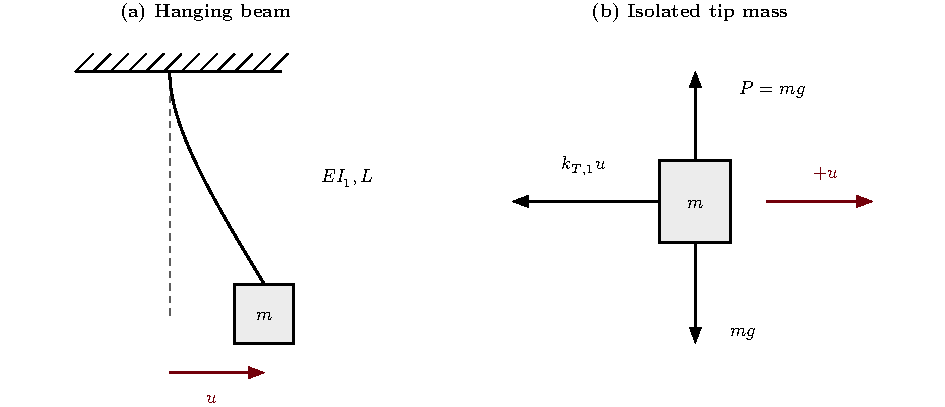
\includegraphics[width=0.95\linewidth,height=0.30\textheight,keepaspectratio,alt={Hanging beam and isolated tip mass showing vertical weight, vertical beam reaction, and horizontal restoring reaction.}]{figures/generated/solutions/flex_pendulum_fbd.pdf}
\caption{C.7.3. Hanging beam and tip-mass free-body diagram. The horizontal restoring reaction includes the effect of tensile preload.}
\end{figure}

Let \(k_{T,1}\) denote the lateral tip stiffness including tensile preload. To first order, the upward beam reaction balances \(mg\), while the horizontal beam reaction is \(-k_{T,1}u\). Newton's law gives
\[
\boxed{\sum F_x=-k_{T,1}u=m\ddot u,\qquad P-mg=0}
\qquad\text{(C.7.4)}
\]
The vertical rise during lateral motion is second order in \(u\). Its gravitational potential energy is nevertheless quadratic and must be retained when deriving the linear restoring stiffness.

To determine \(k_{T,1}\), let \(w(s)\) be the lateral deflection under a horizontal tip force \(H\). The small-slope potential energy, including the tensile preload, is
\[
\Pi[w]=\frac12\int_0^L EI_1(w'')^2\,ds
       +\frac12\int_0^L P(w')^2\,ds-Hw(L).
\]
Primes denote derivatives with respect to \(s\). Stationarity of this energy gives the massless beam equation and boundary conditions,
\[
EI_1w''''-Pw''=0,\qquad w(0)=w'(0)=0,
\]
\[
w''(L)=0,\qquad Pw'(L)-EI_1w'''(L)=H.
\]
Define \(\lambda_1=\sqrt{P/(EI_1)}\). Solving the boundary-value problem gives
\[
w(s)=\frac{H}{P}\left[s-
\frac{\sinh(\lambda_1L)-\sinh\bigl(\lambda_1(L-s)\bigr)}
{\lambda_1\cosh(\lambda_1L)}\right].
\]
At the tip, this reduces to
\[
u=w(L)=\frac{H}{P}\left[L-\frac{\tanh(\lambda_1L)}{\lambda_1}\right].
\]
Thus, the tensile-load stiffness and linearized equation of motion are
\[
\boxed{k_{T,1}=\frac{P}{L-\tanh(\lambda_1L)/\lambda_1},
\qquad P=mg,\qquad\lambda_1=\sqrt{\frac{P}{EI_1}}}
\]
\[
\boxed{m\ddot u+k_{T,1}u=0}\qquad\text{(C.7.5)}
\]
This is the tension-dependent stiffness of a massless cantilever with a tip mass, also given by Likins and Barbera in Appendix II, page 143~\cite{Likins1971Spacecraft}. It is exact within the stated linear, massless-beam model. It does not include finite-deflection geometry, distributed beam inertia, or tip-mass rotary inertia.

The natural frequency follows by dividing the equation of motion by \(m\),
\[
\boxed{\omega_{n,\mathrm{FBP}}=\sqrt{\frac{k_{T,1}}{m}}
=\sqrt{\frac{g}{L-\tanh(\lambda_1L)/\lambda_1}}}
\qquad\text{(C.7.6)}
\]
The normalized governing equation is therefore
\[
\boxed{\ddot u+\omega_{n,\mathrm{FBP}}^2u=0}
\qquad\text{(C.7.7)}
\]

As a consistency check, for \(PL^2/(EI_1)\ll1\), expansion of the hyperbolic tangent gives
\[
k_{T,1}=\frac{3EI_1}{L^3}+\frac{6P}{5L}
+O\!\left(\frac{P^2L}{EI_1}\right).
\]
Consequently, \(k_{T,1}\to3EI_1/L^3\) when the preload vanishes. The leading gravity correction is \(6mg/(5L)\), rather than \(3mg/(2L)\). For large tensile preload relative to bending stiffness, the frequency approaches the simple-pendulum value \(\sqrt{g/L}\) as \(EI_1\to0\).

Problem B.1 has the same undamped single-degree-of-freedom equation after replacing its spring stiffness by \(k_{T,1}\). The roots are \(s_{1,2}=\pm i\omega_{n,\mathrm{FBP}}\), giving
\[
\boxed{u(t)=A\cos(\omega_{n,\mathrm{FBP}}t)
+B\sin(\omega_{n,\mathrm{FBP}}t)}
\qquad\text{(C.7.8)}
\]
Applying \(u(0)=u_0\) and \(\dot u(0)=\dot u_0\) gives \(A=u_0\) and \(B=\dot u_0/\omega_{n,\mathrm{FBP}}\). Hence,
\[
\boxed{u(t)=u_0\cos(\omega_{n,\mathrm{FBP}}t)
+\frac{\dot u_0}{\omega_{n,\mathrm{FBP}}}\sin(\omega_{n,\mathrm{FBP}}t)}
\qquad\text{(C.7.9)}
\]

For major-axis bending, replace \(I_1\) by \(I_2\) throughout the tension-dependent stiffness calculation. The tensile force remains \(P=mg\), but the deflected shape and its effective stiffness change with \(EI_2\). Thus,
\[
\boxed{\begin{aligned}
\lambda_2&=\sqrt{\frac{mg}{EI_2}},&
k_{T,2}&=\frac{mg}{L-\tanh(\lambda_2L)/\lambda_2},\\
\omega_{n,2}&=\sqrt{\frac{k_{T,2}}{m}},&
\frac{I_2}{I_1}&=\left(\frac{b}{h}\right)^2
\end{aligned}}\qquad\text{(C.7.10)}
\]
For \(b>h\), the major-axis motion has the larger frequency and shorter period. When elastic bending stiffness dominates the preload effect for both axes, the frequency ratio approaches \(\sqrt{I_2/I_1}=b/h\). The major-axis initial-value solution follows by replacing \(\omega_{n,\mathrm{FBP}}\) with \(\omega_{n,2}\).
